\documentclass[12pt,fleqn]{book}

\usepackage{titlesec}
\usepackage{caption}

\titleformat{\chapter}[display]
  {\normalfont\huge\bfseries}{}{0pt}{\Huge}
\titlespacing{\chapter}
  {0pt}{10pt}{40pt}

	\newenvironment{amatrix}[1]{%
	  \left[\begin{array}{@{}*{#1}{r}|r@{}}
	}{%
	  \end{array}\right]
	}


\usepackage{amsmath,amssymb,amsfonts,graphicx,tasks,tikz,pgfplots}
\usetikzlibrary{arrows}
\pgfplotsset{compat=1.17}

\usepackage{tasks}
\settasks{
  label-width = 18pt
}
 
\makeatletter
 \def\@textbottom{\vskip \z@ \@plus 1pt}
 \let\@texttop\relax
\makeatother

\usepackage[letterpaper,margin=0.5in,footskip=.5cm]{geometry}

\setlength\parindent{0pt}

\usepackage{amsmath,amssymb,amsfonts,graphicx,tasks,tikz,pgfplots}
\usepackage{amsthm,thmtools}
\usetikzlibrary{arrows,quotes}

\usepackage{array}
\newcommand{\PreserveBackslash}[1]{\let\temp=\\#1\let\\=\temp}
\newcolumntype{C}[1]{>{\PreserveBackslash\centering}p{#1}}
\newcolumntype{R}[1]{>{\PreserveBackslash\raggedleft}p{#1}}
\newcolumntype{L}[1]{>{\PreserveBackslash\raggedright}p{#1}}

% Two-branch graph with equal scale and only max tick labels
% #1 = y1(x), #2 = y2(x), #3 = xmin, #4 = xmax, #5 = ymin, #6 = ymax,
% #7 = tick distance (ignored for equal scale), #8 = extra axis opts, #9 = plot opts
\newcommand{\graphpair}[9]{%
\begin{tikzpicture}[baseline=(current bounding box.north)]
  \begin{axis}[
    axis lines=middle,
    axis line style={very thick},
    grid style={thin,densely dotted,black!50},
    grid=major,
    xmin=#3-.2, xmax=#4+.2,
    ymin=#5-.2, ymax=#6+.2,
    xlabel=$x$, ylabel=$y$,
    axis equal image,
    % Only show largest tick values on each axis
    xticklabels={},
	yticklabels={},
	xtick distance=1, ytick distance=1,
	extra x ticks={#4},
	extra y ticks={#6},
    enlargelimits=false,
    % Allow optional extra axis settings
    #8
  ]
    \addplot[domain=#3:#4, samples=500, #9] (x,{#1});
    \addplot[domain=#3:#4, samples=500, #9] (x,{#2});
  \end{axis}
\end{tikzpicture}%
}


\newcommand{\graph}[8]{
\begin{tikzpicture}[baseline=(current bounding box.north)]
  \begin{axis}[
    axis lines=middle,
    axis line style={very thick},
    grid style={thin,densely dotted,black!50},
    grid=major,
      xtick distance=#6, ytick distance=#6,
      xmin=#2-.2, xmax=#3+.2,
      ymin=#4-.2, ymax=#5+.2,
      xlabel=$x$,
      ylabel=$y$,
    xticklabels={},
	yticklabels={},
	xtick distance=1, ytick distance=1,
	extra x ticks={#3},
	extra y ticks={#5},
      #7]
      \addplot[
      domain=#2:#3,
      samples=500,#8]
      (x,{#1});
    \end{axis}
  \end{tikzpicture}
}

\newcommand{\graphtwo}[9]{
\begin{tikzpicture}[baseline=(current bounding box.north)]
  \begin{axis}[
    axis lines=middle,
    axis line style={very thick},
    grid style={thin,densely dotted,black!50},
    grid=major,
      xtick distance=#7, ytick distance=#7,
\usepackage{amsmath,amssymb,amsfonts,amsthm,thmtools}
      xmin=#3-.2, xmax=#4+.2,
      ymin=#5-.2, ymax=#6+.2,
      xlabel=$x$,
      ylabel=$y$,
      #8]
      \addplot[
      domain=#3:#4,
      samples=500,#9]
      (x,{#1});
      \addplot[
      domain=#3:#4,
      samples=500,#9]
      (x,{#2});
    \end{axis}
  \end{tikzpicture}
}

\newcommand{\curve}[7]{% function, xmin, xmax, ymin, ymax, 
\begin{tikzpicture}[baseline=(current bounding box.north)]
  \begin{axis}[
    axis lines=middle,
    axis line style={very thick},
    grid style={thin,densely dotted,black!50},
    grid=major,
    xticklabels={},
	yticklabels={},
	xtick distance=1, ytick distance=1,
	extra x ticks={#3},
	extra y ticks={#5},
      xmin=#2-.2, xmax=#3+.2,
      ymin=#4-.2, ymax=#5+.2,
      xlabel=$x$,
      ylabel=$y$,
      #6]
      \addplot[
      domain=#2:#3,
      samples=500,#7]
      (x,{#1});
    \end{axis}
  \end{tikzpicture}
}

\newcommand{\blankgraph}[6]{
\begin{tikzpicture}[baseline=(current bounding box.north)]
  \begin{axis}[
    width=#5in,height=#6in,
    axis lines=middle,
    axis line style={very thick},
    grid style={thin,densely dotted,black!50},
    grid=major,
    xticklabels={},
	yticklabels={},
	xtick distance=1, ytick distance=1,
	extra x ticks={#2},
	extra y ticks={#4},
      xtick distance=1, ytick distance=1,
      xticklabels={1},
      yticklabels={1},
      xmin=#1-.2, xmax=#2+.2,
      ymin=#3-.2, ymax=#4+.2,
      xlabel=$x$,
      ylabel=$y$]
    \end{axis}
  \end{tikzpicture}
}

\newcommand{\blankaxes}[2]{
\begin{tikzpicture}[baseline=(current bounding box.north)]
  \begin{axis}[
    width=#1in,height=#2in,
    axis lines=middle,
    axis line style={very thick},
    grid=major,
    xtick distance=2, ytick distance=2,
    xmin=-1, xmax=1,
    ymin=-1, ymax=1,
    xlabel=$x$,
    ylabel=$y$]
  \end{axis}
\end{tikzpicture}
}

\newcommand{\ds}{\displaystyle}

\newcommand{\lr}[1]{\left(#1\right)}

% \usepackage{amsthm}
% \theoremstyle{definition}
% \newtheorem{problem}{}
% \counterwithin*{problem}{section}
% \renewcommand{\theproblem}{\thesubsection.\arabic{problem}}
%
% \newtheorem*{solutionx}{\thesolutionnumber}
% \ExplSyntaxOn
% \tl_new:N \g_gargantuar_solution_tl
%
% \NewDocumentEnvironment{solution}{+b}
%  {
%   \tl_gput_right:Nx \g_gargantuar_solution_tl
%    {
%     \printsolution{\theproblem}{ \exp_not:n { #1 } }
%    }
%  }
%  {}
% \NewDocumentCommand{\printsolutions}{}
%  {
%   \tl_use:N \g_gargantuar_solution_tl
%   \tl_gclear:N \g_gargantuar_solution_tl
%  }
% \NewDocumentCommand{\printsolution}{m +m}
%  {
%   \cs_set:Npn \thesolutionnumber { #1 }
%   \begin{solutionx} #2 \end{solutionx}
%  }
% \ExplSyntaxOff
% \makeatother
%
% \newcommand{\prb}[1]{\begin{problem}#1\end{problem}}
% \newcommand{\sol}[1]{\begin{solution}#1\end{solution}}
% =============================
% TCOLORBOX CONFIGURATION
% =============================

\usepackage{tcolorbox}

\definecolor{black}{rgb}{0,0,0}
\definecolor{dark-gray}{rgb}{.15,.15,.15}
\definecolor{light-gray}{rgb}{.85,.85,.85}
\definecolor{white}{rgb}{1,1,1}

\makeatletter
\newcommand*\ifcounter[1]{%
	\ifcsname c@#1\endcsname
		\expandafter\@firstoftwo
	\else
		\expandafter\@secondoftwo
	\fi
}
\makeatother

\tcbuselibrary{theorems}

\ifcounter{unit}{
	\newtcbtheorem{defn}{Definition \theunit.\hspace{-.3em}}{
		colback=light-gray,colframe=dark-gray,coltitle=white,coltext=black,fonttitle=\bfseries,before skip=20pt plus 2pt,after skip=20pt plus 2pt}{th}
}{
	\newtcbtheorem{defn}{Definition}{
		colback=light-gray,colframe=dark-gray,coltitle=white,coltext=black,fonttitle=\bfseries,before skip=20pt plus 2pt,after skip=20pt plus 2pt}{th}
}

\ifcounter{unit}{
	\newtcbtheorem{thm}{Theorem \theunit.\hspace{-.3em}}{
		colback=light-gray,colframe=dark-gray,coltitle=white,coltext=black,fonttitle=\bfseries,before skip=20pt plus 2pt,after skip=20pt plus 2pt}{th}
}{
	\newtcbtheorem{thm}{Theorem}{
		colback=light-gray,colframe=dark-gray,coltitle=white,coltext=black,fonttitle=\bfseries,before skip=20pt plus 2pt,after skip=20pt plus 2pt}{th}
}



\pagestyle{plain}
\usepackage[lastexercise,answerdelayed]{exercise}
\usepackage{totcount}
\regtotcounter{Exercise} % register the counter for getting the total
\usepackage{chngcntr}
\counterwithin{Exercise}{chapter}
\counterwithin{Answer}{chapter}
\usepackage{xassoccnt}
\NewTotalDocumentCounter{totalex}
\usepackage{titleref}
\usepackage{etoolbox}

%EXERCISE START

\renewcommand{\ExerciseHeader}{ \stepcounter{totalex}\ifnumcomp{\value{Exercise}}{=}{1}{\ifnumcomp{\thechapter}{=}{1}{}{\vspace{10pt}}\noindent\Large\textbf{Exercises}\par\vspace{10pt}}{}\noindent\normalsize\bfseries\ExerciseHeaderNB\ExerciseHeaderDifficulty.}
\renewcommand{\AnswerHeader}{\ifnumcomp{\value{Exercise}}{=}{1}{\ifnumcomp{\thechapter}{=}{1}{}{\vspace{10pt}}\noindent\Large\textbf{Section\ \thechapter\ Solutions}\par\vspace{10pt}}{}\noindent\normalsize\bfseries\ExerciseHeaderNB.\ }

\usepackage{hyperref}

\newcommand{\prb}[1]{\begin{Exercise}#1\end{Exercise}}
\newcommand{\sol}[1]{\begin{Answer}#1\end{Answer}}

\begin{document}
\noindent
\thispagestyle{empty}
Grade 10 Advanced Math \hfill Name: \hspace{2in}
\medskip\hrule
\noindent

\vfill

\begin{center}
	{\bf \huge Chapter 3: Radicals and Exponents}
\end{center}

\vfill
\vfill

\clearpage

\setcounter{page}{1}

{\bf \huge Introduction }
\\[1in]
In the first chapter, we dealt with functions that could be sketched as a straight line.  We observed how they intersected with each other, and how we can use algebra to describe those intersections.
\\[1em]
In the second chapter, we learned about polynomial functions, namely quadratics, and how they can be graphed.  We spent a great deal of time finding roots of a quadratic, and even learned about imaginary numbers.
\\[1em]
In this chapter, we will learn about the inverse of a quadratic -- a radical.  We will learn how to play with these kinds of numbers, what \emph{kinds} of numbers they can be, and how to express them in various ways.
\\[1em]
Try this warm up to see if you can get all of these facts right.
\begin{tasks}(2)
    \task $3^2=$
    \task $(-3)^2=$
    \\[1em]
    \task If $x^2=9,$ then $x=$
    \task $\sqrt 9 =$
    \\[1em]
    \task $\sqrt{x^2}=$
    \task $(\sqrt x)^2=$
\end{tasks}
\clearpage
\chapter{1. Relations, Functions, One-to-one}
We have seen several types of function in this class so far.  The first type, and most straightforward was the linear function.  Then we realized that if we multiplied two linear functions together, we got a quadratic function.  There are also higher-degree polynomial functoins that we briefly explored in the last chapter.
\\[1em]
It turns out that functions are the life-blood of a lot of mathematics.  Most of mathematics can be described using the language of functions.
\\[1em]
But not all equations can be described as a function.  It is probably a  good idea to remind ourselves what exactly a function is!
\begin{defn}{Function}{}
A function is a rule that takes as input one value and outputs another value, related to the input.  If $x$ is the input of function $f$, and $y$ is the output of the function, then we write
\[
    y=f(x)
\]
\end{defn}
It is critical to understand that for every single input, there is a single output.  A function fails to be a function if you were to input a single value and get back \emph{two} or more values.
\\[1em]
Consider the following functions.
\begin{tasks}(4)
    \task
    $f(x)=x^2$
    \task
    $f(x)=(x-2)(x+1)^2$
    \task
    $y=x-4$
    \task
    $g(x)=\sqrt x$
\end{tasks}
Use Desmos to help you graph the above functions below.
\\[1em]
\blankgraph{-4}{4}{-4}{4}{2.3}{2.3}
\blankgraph{-4}{4}{-4}{4}{2.3}{2.3}
\blankgraph{-4}{4}{-4}{4}{2.3}{2.3}
\blankgraph{-4}{4}{-4}{4}{2.3}{2.3}
\\[1em]
Some equations in math, however, are not best described as a function.  Sometimes if I give you one input, you may want two outputs.
\\[1em]
The following are not functions:
\begin{tasks}(2)
    \task
    $y^2=x$
    \task
    $x^2+y^2=1$
    \task
    $x^3+y^2=xy$
    \task
    $y=\pm x$
\end{tasks}
Use Desmos to help you graph these functions.  Try to see if you can visualize \emph{exactly} what makes these equations non-functions.
\\[1em]
\blankgraph{-4}{4}{-4}{4}{2.3}{2.3}
\blankgraph{-4}{4}{-4}{4}{2.3}{2.3}
\blankgraph{-4}{4}{-4}{4}{2.3}{2.3}
\blankgraph{-4}{4}{-4}{4}{2.3}{2.3}
\\[1em]
\begin{defn}{Relation}{}
    An equation that has two or more variables is called a relation.  Most relations are between two variables, $x$ and $y$.  If the relation $R$ has a solution $x=a$ and $y=b$, then the the relation can be graphed by plotting $(a,b)$, and all other solutions to the equation.  Furthermore, we can write $a R b$ and say $a$ is related to $b$.
\end{defn}
So all of the above equations are relations because they represent a relationship between $x$ and $y$.  When Desmos graphs these, they are finding all possible solutions to the equation, and plotting each point, one by one.
\\[1em]
There is a quick way of determining when a graph represents a function and when it doesn't.  
\begin{defn}{Vertical Line Test}{}
Given the graph of a relation, if there exists a vertical line that overlaps the curve of the graph more than once, then the relation is not a function.  If no such vertical line exists, then the relation is a function.
\end{defn}
Use the Vertical Line Test to determine which of these graphs represents a relation that is a function, and which is a relation that is \emph{not} a function.
\begin{tasks}(2)
\task \graph{0.2*(x + 2)*(x - 1)*(x - 3)}{-4}{6}{-6}{6}{1}{}{}
\task \graphpair{1 + 3*sqrt(1 - (x/2)^2)}{1 - 3*sqrt(1 - (x/2)^2)}{-2}{2}{-2.5}{4.5}{0.5}{}{}
\task \graphpair{2}{-(2 - (x - 1)^2)}{-3}{5}{-4}{4}{1}{}{}
\task \graph{(x - 1)^2 - 2}{-4}{6}{-4}{6}{1}{}{}
\task \graph{abs(x)}{-5}{5}{-1}{5}{1}{}{}
\task \graphpair{sqrt(9-x^2)}{-sqrt(9-x^2)}{-3}{3}{-3}{3}{1}{}{}
\task \graph{-0.5*x + 2}{-6}{6}{-4}{6}{1}{}{}
\task \graphpair{1 + sqrt(x + 2)}{1 - sqrt(x + 2)}{-2}{7}{-3}{5}{1}{}{}
\end{tasks}

As you may be able to sense, a function is a special type of relation.  But is there something even more special?  Are there types of functions are even more exclusive?  It turns out: yes.  These functions are called one-to-one functions.

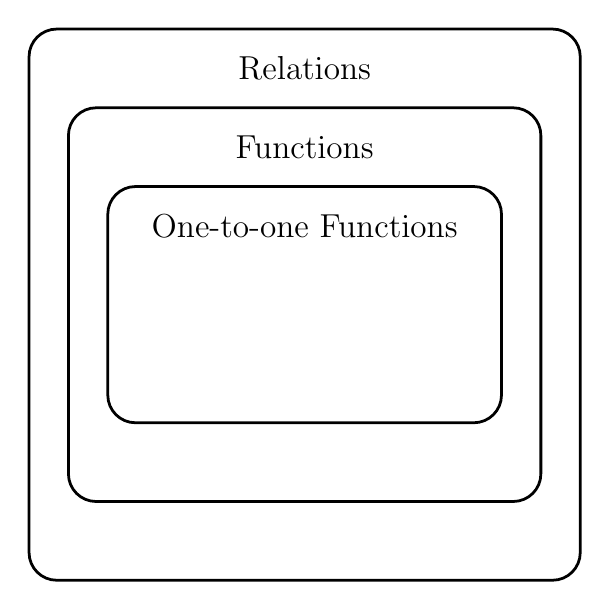
\begin{tikzpicture}[font=\large, line width=1pt]

% Outer rectangle: Relations
\node[draw, rounded corners=10pt, minimum width=7cm, minimum height=7cm, anchor=center] (relations) at (0,0) {};

% Middle rectangle: Functions
\node[draw, rounded corners=10pt, minimum width=6cm, minimum height=5cm, anchor=center] (functions) at (0,0) {};

% Inner rectangle: One-to-one Functions
\node[draw, rounded corners=10pt, minimum width=5cm, minimum height=3cm, anchor=center] (one2one) at (0,0) {};

% Labels (placed near the top of each rectangle)
\node at (0,3) {Relations};
\node at (0,2) {Functions};
\node at (0,1) {One-to-one Functions};

\end{tikzpicture}

\chapter{2. Inverse Functions}
\chapter{3. The Radical Function}
\chapter{4. Number Systems}
\chapter{5. Manipulating Radicals}
\chapter{6. Factoring}
\chapter{7. Exponential Notation}
\chapter{8. Logarithms}
\prb{a problem}
\sol{a solution}
\chapter{Selected Solutions.}
\shipoutAnswer
\end{document}
